%%%%%%%%%%%%%%%%%%%%%%%%%%%%%%%%%%%%%%%%%%%%%%%%%%%%%%%%%%%%%%%%%%%%%%%%
% Preamble
%%%%%%%%%%%%%%%%%%%%%%%%%%%%%%%%%%%%%%%%%%%%%%%%%%%%%%%%%%%%%%%%%%%%%%%%
\documentclass[12pt]{article}
%
% Packages and other includes
% Pagination
\usepackage[letterpaper, margin=1in]{geometry}

%
% Graphics, floats, tables
\usepackage{graphicx, xcolor, float, array}
\graphicspath{{image/}}
%
% Fonts
\usepackage[T1]{fontenc} % best for Western European languages
\usepackage{lmodern} % Latin Modern instead of CM
\usepackage{textcomp} % required to get special symbols
%
% Math
\usepackage{amsmath, amssymb}
\usepackage{enumerate}
\usepackage{braket}
% 
% Hyperlinks
\usepackage[colorlinks,linkcolor={red},citecolor={blue},
urlcolor={blue}]{hyperref} 
%
% Definitions and settings
% Paragraph indent and spacing
\setlength{\parskip}{0.4\baselineskip}
\setlength{\parindent}{0in}
%
% Math mode version of "r" column type (requires array package)
\newcolumntype{R}{>{$}r<{$}}
\newcommand{\brian}[1]{{\color{orange}{#1}}}
% Title, authors, date
\title{\textbf{Homework 1}}
\date{\vspace{-2em}\today}

\begin{document}

\maketitle 

Weekly homework assignments are posted approximately one week prior to the
due date. Collaborations are encouraged and students must report all collaborators
in writing on each assignment. All external sources (websites, books) must be
properly cited. Additional problems are listed at the end of each assignment.
This week's assignment is due \textit{Tuesday, Sept 6th at 10:00am.}

\textbf{One More Time: Significant Figures and Unit Conversion}

1) Calculate the following with the proper number of significant figures. (2 pts)

\begin{enumerate}[a)]
\item \begin{equation*}
  \frac{35.89 \text{g}}{5.5 \text{cm}^3} - \frac{1.86 \text{g}}{(2.259 \text{cm})^3}
\end{equation*}
\item \begin{equation*}
  \frac{7.291\times 10^5 - 2.139 \times 10^4}{8.5 \times 10^2}
\end{equation*}
\item \begin{equation*}
  (2.998 \times 10^8 \text{m/s})\times(65\text{s}) + 1.45\times 10^9 \text{m}
\end{equation*}
\item \begin{equation*}
  \frac{3.840\times 10^{-3}}{(7.25\times 10^2)(0.087)}
\end{equation*}
\end{enumerate}

2) Cow farts realease methane, which is a major contributor to the growing greenhouse
gases in the atmosphere. A cow releases approximately 320 L of methane per day.
The world is home to 1.5 billion cows. How much methane is released into the
atmosphere in one day, one week, and one year? The Earth's atmosphere is approximately
$5.18\times 10^{19}$ m$^3$. What is the percentage of the total yearly released methane
relative to Earth's atmosphere? (3 pts)

\vspace{2in}

\textbf{Matter and Its Classification}

2) Classify each of the following as an element or a compound: S$_8$(s), O$_2$(g),
H$_2$O(l), P$_4$, He, and C(diamond). (1 pt)

\vspace{0.5in}

3) Based on the image, rank the density liquids and solids. In your own words,
explain why you rank the density of the materials that way. (2 pts)

\begin{center}
  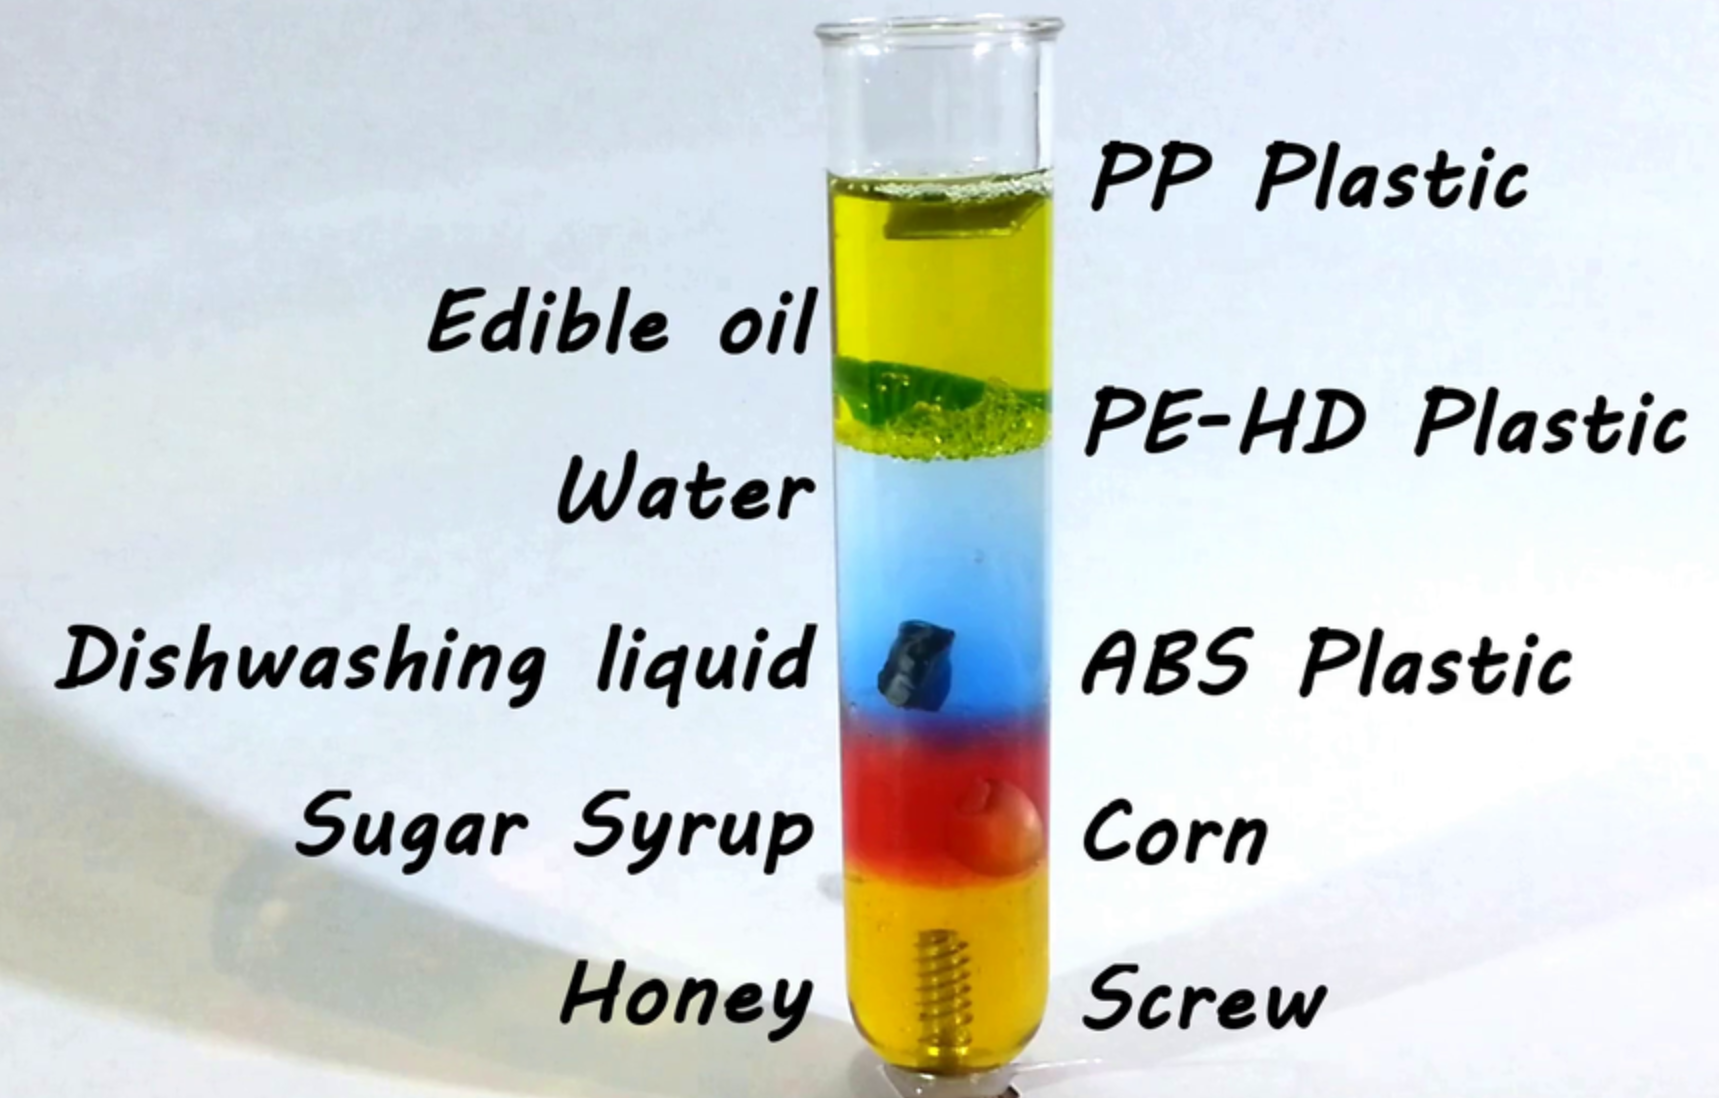
\includegraphics[scale=0.12]{dens_liq_sol}
\end{center}

\vspace{1in}

\textbf{Periodic Table}

4) Isotopes are atoms that have the same number of proton and different number of
neutrons. The common notation is as follows,
\begin{equation*}
  ^\text{A}_\text{Z}\text{X},
\end{equation*}
where A is the mass number, Z is the atomic number, and X is the atomic symbol.
Suppose an element with three stable isotopes has 82 protons. The separate isotopes contain 124,
125, and 126 neutrons. Identify the element and write symbols for the isotopes. (2 pts)

\vfill

\textbf{Optional Textbook Problems:} Ch. 1- $1.3-1.59$ odd, $1.85-1.99$ odd, 1.114

\end{document}
